\documentclass[14pt]{extarticle}
\usepackage[utf8]{inputenc}
\usepackage[T1]{fontenc}
\usepackage[spanish,es-lcroman]{babel}
\usepackage{amsmath}
\usepackage{amsthm}
\usepackage{physics}
\usepackage{tikz}
\usepackage{float}
\usepackage{calc}
\usepackage[autostyle,spanish=mexican]{csquotes}
\usepackage[per-mode=symbol]{siunitx}
\usepackage{gensymb}
\usepackage{multicol}
\usepackage{enumitem}
\usepackage{setspace}
\usepackage[left=2.00cm, right=2.00cm, top=2.00cm, 
     bottom=2.00cm]{geometry}
\usepackage{Estilos/ColoresLatex}
\usepackage{makecell}

\newcommand{\textocolor}[2]{\textbf{\textcolor{#1}{#2}}}
\sisetup{per-mode=symbol}
\decimalpoint
\sisetup{bracket-numbers = false}
\newlength{\depthofsumsign}
\setlength{\depthofsumsign}{\depthof{$\sum$}}
\newcommand{\nsum}[1][1.4]{% only for \displaystyle
    \mathop{%
        \raisebox
            {-#1\depthofsumsign+1\depthofsumsign}
            {\scalebox
                {#1}
                {$\displaystyle\sum$}%
            }
    }
}


\author{\normalsize{M. en C. Gustavo Contreras Mayén.} \quad \normalsize{\texttt{gux7avo@ciencias.unam.mx}} \\
\normalsize{M. en C. Abraham Lima Buendía.} \quad \normalsize{\texttt{abraham3081@ciencias.unam.mx}}}
\title{\vspace*{-2cm} Tarea 1 - Curso de Óptica}
\date{ }

\begin{document}

\setstretch{1.3}

\maketitle
\fontsize{14}{14}\selectfont

\textbf{Indicaciones: } Presenta de manera ordenada y con el mayor detalle posible la solución a cada uno de los ejercicios. La tarea se entrega en físico en el salón de clase, ocupa las hojas que consideres, anotando tu nombre en cada de una de ellas, numera también las hojas.

\textbf{Fecha de entrega: } \underline{\textbf{Lunes 11 de marzo al inicio de la clase}}. 

\begin{enumerate}
\item Demostrar que el momento canónico del campo electromagnético en el vacío es: $\va{p} = \epsilon_{0} \, \mu_{0} \, \va{S}$
\item Bajo las consideraciones: $0\leq x\leq a$, junto con $H_{0},\, a, \, k$ y $\omega$ son constantes y que se satisface la relación de dispersión $\mu_{0} \, \epsilon_{0} \, \omega^{2} = k^{2} + \left( \dfrac{\pi}{a} \right)^{2}$.

a) Demuestra que las siguientes expresiones:
\begin{align*}
E_{y} &= -H_{0} \, \mu_{0}\, \omega \, \left(\dfrac{a}{\pi}\right) \, \sin \left( k \, z - \omega \, t \right) \, \sin \left(\dfrac{\pi \, x}{a} \right) \\
H_{x} &= H_{0} \, k \, \left(\dfrac{a}{\pi}\right) \, \sin \left(k \, z - \omega \, t\right) \, \sin \left(\dfrac{\pi \, x}{a}\right) \\
H_{z} &= H_{0} \, \cos \left(k \, z - \omega \, t \right) \, \cos \left(\dfrac{\pi \, x}{a} \right)
\end{align*}
satisfacen las ecuaciones de Maxwell en el vacío. El resto de las componentes son cero y puedes asumir que no hay presencia de cargas o corrientes libres.

b) Encuentra la corriente de desplazamiento.

c) Encuentra el vector de Poynting.
\item Una onda estacionaria viene dada por:
\begin{align*}
E = 100 \, \sin \left( \dfrac{2}{3} \, \pi \, x \right) \, \cos \left( 5 \, \pi \, t \right)
\end{align*}
determina dos ondas que pueden superponerse para crearla.
\item Demuestra que la representación de Fourier de la función $f (x) =\abs{\sin (x)}$ es:
\begin{align*}
f (x) = \dfrac{2}{\pi} - \dfrac{4}{\pi} \nsum_{m=1}^{\infty} \dfrac{\cos (2 \, m \, x)}{4 \, m^{2} - 1}
\end{align*}
\item Describe detalladamente el estado de polarización de cada una de las siguientes ondas:
\begin{enumerate}[label=\roman*)]
\item $\vb{E} = \vu{i} \, E_{0} \, \cos \left( k\, z - \omega \, t \right) - \vu{j} \, E_{0} \, \cos \left( k \,z - \omega \, t \right)$
\item $\vb{E} = \vu{i} \, E_{0} \, \sin \left( 2 \, \pi \left[ \dfrac{z}{\lambda} - \nu \, t\right] \right) - \vu{j} \, E_{0} \, \sin \left( 2 \, \pi \left[\dfrac{z}{\lambda} - \nu \, t \right]\right)$
\item $\vb{E} = \vu{i} \, E_{0} \, \sin \left(\omega \, t - k \, z \right) + \vu{j} \, E_{0} \, \sin \left( \omega \, t - k \, z - \dfrac{\pi}{4} \right)$
\item $\vb{E} = \vu{i} \, E_{0} \, \cos \left( \omega \, t - k \, z \right) + \vu{j} \, E_{0} \, \cos \left( \omega \, t - k \, z + \dfrac{\pi}{2} \right)$
\end{enumerate}
\item Las longitudes de onda de dos ondas \textit{A} y \textit{B} son de \SI{500}{\nano\meter} en el vacío, el tanque de vidrio $( n = 1.52)$ se llena con agua $(n = 1.33)$, si las ondas comienzan en fase y todos los números anteriores son exactos, encuentra su diferencia de fase relativa en la línea de meta (se presenta a continuación un esquema del problema).
\begin{figure}[H]
    \centering
    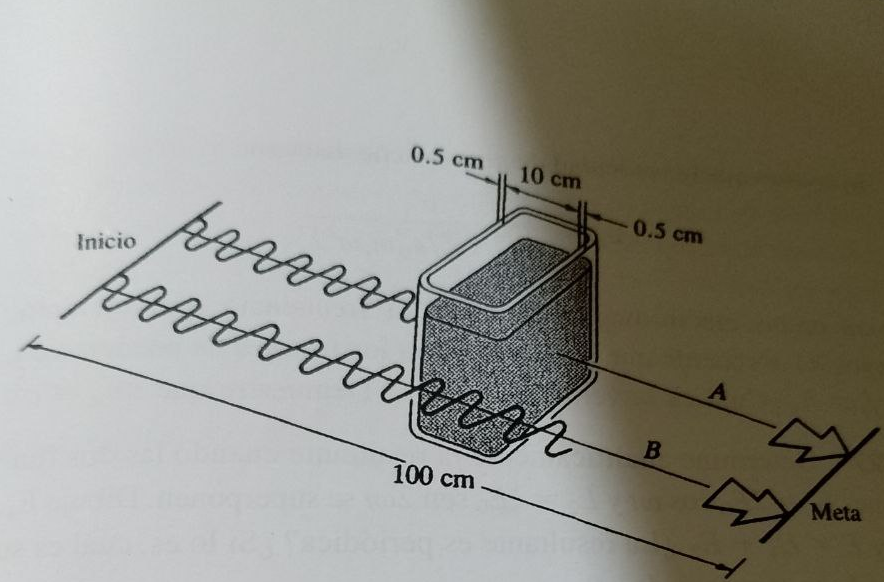
\includegraphics[scale=0.5]{tarea 1.png}
\end{figure}
\end{enumerate}

\end{document}